% arara: pdflatex
%Began 17 August 2024 --- 
\documentclass[a4paper,x11names,svgnames,10pt]{article}
\usepackage{amsmath}
\usepackage{hyperref}
% the \hypersetup{keyvals} commented out below is stored in an external hyperref.cfg file
% to enable the pagebackref=true option
%\hypersetup{%dvips, % not needed for  pdflatex
%	pagebackref=true,
%	pdfauthor={Iam The Author},
%	hyperfigures,
%	bookmarks=true,
%	bookmarksnumbered=true,
%	bookmarksopen=true,
%	colorlinks=true, %if true, link borders absent
%	pdfborder={1 1 1},
%	citecolor=blue,
%	linkcolor=blue,
%	urlcolor=blue,
%}
\usepackage{url}
\usepackage{svg}
\usepackage[utf8]{inputenc}
\usepackage{graphicx}
\usepackage{xcolor}
\usepackage{float}
\usepackage{natbib}

\topmargin -0.50in
\oddsidemargin 0.0in
\textwidth 6.27in
\textheight 9.75in

%%%-----------------------------------------------------
%%% TO BE EDITED FOR EACH NEW SERIES or VOLUME GENERATED 
%%%-----------------------------------------------------
	\def\authorName{I Am The Author}
	\def\authorFirstMidNameInit{I.\ T.\ }
	\def\authorLastName{Author}
	\def\dateGenerated{\today}
	\def\volNumber{I}
	\def\mdgBookTitle{Musical Dice Game - \\[0.15cm] Scottish Dances \volNumber}
	\def\mdgBookSubTitle{{\small based on}\\ Kunst, Schottische Taenze zu componiren, ohne musicalisch zu sein, dargestellt in einer W\"{u}rfel- und Noten-Tabelle, nebst Anleitung  (1830?) \\[0.15cm] by Gustav Gerlach}
	\def\theBookSeries{Wonders of the Musical World Series 6}
	\def\theBookPublisher{Libre Edition Press}
	\def\theBookPublisherLogo{../images/1ed.png}
	\def\theBookFrontCover{../images/FrontCover.pdf}
%%%-----------------------------------------------------
%%%

\def\uline{\underline}
%\definecolor{orange}{rgb}{1,0.5,0} % RGB
%\definecolor{light-gray}{gray}{0.95} % shades
%\definecolor{orange}{cmyk}{0,0.5,1,0} % CMYK

\newcommand{\HRule}{\rule{\linewidth}{0.5mm}}

\setlength{\parindent}{0pt}

\DeclareGraphicsExtensions{.pdf,.png}

\setcitestyle{authoryear,round,comma,aysep={,},yysep={,},notesep={, }}

\title{\textsc{\mdgBookTitle}}
\author{\textsc{\authorFirstMidNameInit \authorLastName}}
\date{\textsc{\dateGenerated}}
% ---

\begin{document}

% Book Cover
% File name: mdgBooSV6v1-cover.tex
% Purpose: Book Cover
% Instruction: Should be \input{.} just after \begin{document}
{
\topmargin 0.00in
\oddsidemargin 0.45in
\textwidth 8.27in %letterpaper: 8.50in
\textheight 11.69in %letterpaper: 11.50in
\thispagestyle{empty}

\begin{titlepage}

\begin{picture}(0,0)%
\linethickness{67.00pt}
\color{blue!22!black}
\put(-105,85){\line(1,0){6477}}
\put(-105,-830){\includegraphics[clip=true,trim=0.00in 0.65in 0.25in 0.0in,height=12.50in,width=8.60in,keepaspectratio]%
	{\theBookFrontCover}}
\put(-105,-692){\line(1,0){6477}}
\end{picture}

\vspace{-1.5in}

\begin{center}
	\LARGE\textbf{\color{white} \hspace{-0.5in}\theBookSeries}
\end{center}


\vspace*{1.00\baselineskip}
\begin{center} \Huge\textbf{\color{MediumBlue!1!MidnightBlue}\em \mdgBookTitle}
\end{center}

\vspace{-0.20in}
\begin{center}
	\Large\textbf{\color{MediumBlue!50!MidnightBlue}\em \mdgBookSubTitle}
\end{center}

\begin{center}
	\LARGE\textbf{\color{MediumBlue!25!MidnightBlue}\em compiled by \authorFirstMidNameInit \authorLastName}
\end{center}

\vfill
\begin{center}
	\LARGE\textbf{\hspace{-0.5in}\color{white}\em \theBookPublisher \\ \vspace{-.19in}}
\end{center}
\end{titlepage}
}




\newpage
% Title Page
{
${}_{}$\\
\vspace{1.00in}	
\thispagestyle{empty}
\begin{center}
	\HRule \\[0.4cm]
	{\huge \bfseries \mdgBookTitle} \\[0.2cm]
	{\large{\em \mdgBookSubTitle} }\\[0.2cm]
	\HRule \\[1.5cm]
	% Author and supervisor
	\begin{minipage}{0.4\textwidth}
		\begin{flushleft} \large
			\emph{Author:}\\
			\authorFirstMidNameInit \textsc{\authorLastName}
		\end{flushleft}
	\end{minipage}
	\begin{minipage}{0.4\textwidth}
		\begin{flushright} \large
			\emph{Supervisor:} \\
			Dr. Communio \textsc{Sanctorum}
		\end{flushright}
	\end{minipage}
	\vfill
	% Bottom of the page
	{\textsc{\Large \theBookSeries}}  \\[0.2cm] 
	\includegraphics*[width=0.15\linewidth]{\theBookPublisherLogo}\\ 
	{\large \theBookPublisher \\
       \dateGenerated }\\
	\vspace{2.50in}
\end{center}
\newpage

%\maketitle		% uncomment if no Front Cover

\tableofcontents\label{tabofcon}

%\extrafloats{182}

\baselineskip 14pt

\newpage
\section[Introduction]{Introduction\footnote{The information contained in the introduction were culled from the following online resources:
	\citet{gg1830}, 
	\citet{wiki_mw2017},
	\url{https://opus-infinity.org/}, and 
	\href{https://www.sciencenews.org/article/mozarts-melody-machine-0}{Mozart's Melody Machine} \citep*{peterson2001}
	}
}
	\begin{center}
	\begin{minipage}{0.4\textwidth}
	\begin{flushleft}
		\begin{center}
			``\small Kunst, Schottische Taenze zu componiren, \\
			ohne musicalisch zu sein, \\
			dargestellt in einer Würfel- und \\
			Noten-Tabelle, nebst Anleitung"
		\end{center}
	\end{flushleft}
	\end{minipage}
	\begin{minipage}{0.4\textwidth}
	\begin{flushright}
		\begin{center}
		``\small The art of writing Scottish dances [schottisches/reels], \\
		without having to be musically gifted, \\
		presented in a Dice and \\ 
		Notes Table, with an introduction"
	\end{center}
	\end{flushright}
	\end{minipage}
	\end{center}

Thus run the German title (and its English translation) of the Musical Dice Game (MDG) invented by Gustav Gerlach.  Rightly and interestingly so, as the Rules provided in the published work allow a non-professional musician to generate (``compose") nearly three (3) trillions of unique MDG Scottish Dances (SDs).  More precisely, the rules of the {\it Schottische Taenze}, as we would refer to this MDG from here onward, yields $6^{8} \times 6^{8} = 2,\!821,\!109,\!907,\!456$ unique SDs (see explanation in Subsection~\ref{tabFind}).\\  % Total: (9^6)^2 = 282,429,536,481

A {\it Musikalisches W\"{u}rfelspiel} (German for ``musical dice game" or MDG) is a system for randomly ``generating" (e.g., by using a die or two dice) musical compositions from precomposed options and was quite popular throughout Western Europe in the 18th century.  The earliest known MDG is Johann Philipp Kirnberger's {\em Der allezeit fertige Polonoisen- und Menuettencomponist (1st ed.\ 1757; rev.\ 2nd ed.\ 1783)} (translated from German as ``The Ever-Ready Minuet and Polonaise Composer").  Other well-known composers that are to known to have composed a MDG are C.P.E.\ Bach ({\em Einfall, einen doppelten Contrapunct in der Octave von sechs Tacten zu machen, ohne die Regeln davon zu wissen (1758)}; translated from German as ``A method for making six bars of double counterpoint at the octave without knowing the rules"), Abb\'{e} Maximillian Stadler ({\em Table pour composer des minuets et des Trios \`{a} la infinie; avec deux dez \`{a} jouer (1780)}; translated from French as ``A table for composing minuets and trios to infinity, by playing with two dice"), the latter MDG being also attributed to Franz Joseph Haydn. \\

Probably the most famous of MDGs is {\it Musikalisches W\"{u}rfelspiel K. 516f (1787)}.  This MDG was first published by J.J. Hummel in 1793 in Berlin and was republished in 1796 by Nikolaus Simrock in Bonn (as K. 294d or K. Anh. C 30.01). Simrock attributed this work to Wolfgang Amadeus Mozart. It is also known under the title of {\em Anleitung zum Componieren von Walzern so viele man will vermittelst zweier W\"{u}rfel, ohne etwas von der Musik oder Composition zu verstehen} (German for ``Instructions for the composition of as many waltzes as one desires with two dice, without understanding anything about music or composition") and may have been based on Mozart's manuscript {\em K.\ 516f}, written in 1787, consisting of numerous two-bar fragments of music, that appear to be some kind of game or system for constructing music out of two-bar fragments, but contains no instructions nor hints as to the use of dice.  An \href{(http://www.asahi-net.or.jp/\~rb5h-ngc/e/k516f.htm}{online article} by Hideo Noguchi offers a possible explanation for this attribution. \\

This book is a collection of 20 MDG Scottish Dances that were generated according to the rules given in {\it Schottische Taenze}. The scores of the generated SDs, that were initially written using the \texttt{abc} environment of Chris Walshaw, were converted to Scalar Vector Graphics (SVG) images (with corresponding MIDIs) using {\tt abcm2ps} and {\tt abcmidi}, and were then pre-processed with Inkscape to be included in \LaTeX\ to produce this book.


\section{\em Schottische Taenze}

\subsection{Rules}\label{mdgRules}

The Rules provided in {\em Schottische Taenze} generate SDs consisting of exactly 32 bars (or mesaures) that are divided equally into two (2) main parts: a Dance and a Trio.  The two sets of eight (8) bars for each of the two main parts are played with repeats.  After the Trio is played, the 16 bars of the Dance are again played without repeats, yielding a total of 80 bars of music played for each MDG SD. \\

The following Rules may be followed for generating each SD (not exactly the same as given in the {\it Schottische Taenze}):

\begin{enumerate}
	\item [1.] For each main part (Dance or Trio), toss a usual six-sided die eight times then obtain the numbers on the face that comes up on each toss.  Hence, 16 six-sided one-die tosses (with possible outcomes from the set \{1, 2, 3, 4, 5, 6\} for each toss) are needed to generate a SD. (Two or four six-sided dice may also be used, what is essential is that eight (8) random integers (chosen from 1-6) are generated for constructing the 16 bars of the Dance part; ditto, for the Trio part.)
	\item [2.\label{step2}] The 16 bars for the Dance part are obtained based on the first eight (8) 1-die tosses from Step~1.  The outcome of the first 1-die toss is used for determining the notes for the first two (2) bars of the Dance based on the Table for Measure Numbers (Table~\ref{tabFind}) corresponding to this particular toss and the notes for these two bar numbers given in the Table for Measures (Table~\ref{tabMeas}).\\
	For example, suppose the first 1-die toss (for the Dance part) comes up a 2. The  Table for Measure Numbers (see Table~\ref{tabFind}) leads us to use bar {\tt 77} and bar {\tt 109} from the Table for Measures (Table~\ref{tabMeas}) for creating the 1st and 2nd bars, respectively, of this Dance part.  Thus, the G-clef notes and F-clef notes for the first bar of this Dance part being that is being constructed are: {\tt [Ec][Ec] [Fd][Ge]; C,C [B,C][\_B,C]} (in {\tt abc} notation), while those for the second bar of this Dance part that is being constructed are: {\tt !turn!f3/g/a2 \& A4; C4 \& A,3/G,/ F,2}. 

	\item[3.\label{step3}] Step~2.\ is repeated for the outcomes of the remaining seven (7) 1-die tosses from Step 1., eventually leading to the completion of the 16 bars of the Dance part. Thus, the outcome of the second 1-die toss from Step~1.\ is used for determining the notes for the 3rd and 4th bars of this Dance part that is being constructed, that of the 3rd 1-die toss for the 5th and 6th bars, and so forth, until the outcome of the 8th 1-die toss, which is used for determining the notes for the 15th and 16th bars of this Dance part that is being constructed. 
	
	\item[4.] The remaining eight (8) tosses of the 16 tosses from Step~1.\ are similarly used to find the notes for the 16 bars of the second main part (the Trio) in a manner similar to that described in Steps~2.\ and 3.\ above for the first main part (the Dance).
\end{enumerate}   

\subsection{Table for finding Measure Number from Table of Measure Numbers}\label{tabFind}
The table given here (Table~\ref{fig:0tab1}) combines the two (2) tables given on page 3 of {\it Schottische Taenze}.  The leftmost column contains the possible die outcomes (which are precisely the integers from 1 to 6 as we are tossing an ordinary six-sided die) while the topmost row contains the bar numbers (16 + 16 = 32 in all) for the MDG SD (Dance with Trio) to be generated---16 bars for the first main part (Dance) and also 16 bars for the second main part (Trio).\\

The body of Table~\ref{fig:0tab1}(a) and (b) includes $\underbrace{6 \times 16}_{\tt Dance} \;+\;$ $\underbrace{6\times 16}_{\tt Trio} \;=\;$ $6\times 32 \;=\; 192$ measure numbers, which is also the total number of measures that appear in the Table of Measures for the Dances and Trios (Figures~\ref{fig:meas1} to \ref{fig:meas4}).  Since eight (8) one-die tosses determine a unique sequence of 16 bars for a Dance part and each 1-die toss has exactly six (6) possible outcomes, then the total number of 16-bar Dance parts that can be constructed based on the Rules in Section~\ref{mdgRules} is $6^{8} = 1,679,616$ (approximately 1.68 million). Similarly, the total number of 16-bar Trio parts that can be constructed based on the Rules in Section~\ref{mdgRules} is $6^{8} = 1,679,616$.  Thus, the total number of unique MDG SDs based on {\em Schottische Taenze} is $6^{8} \times 6^{8} = 2,\!821,\!109,\!907,\!456$ (nearly 3 trillions). \\


\begin{table}[H]
	\centering
	\begin{tabular}{c}
		\centering
		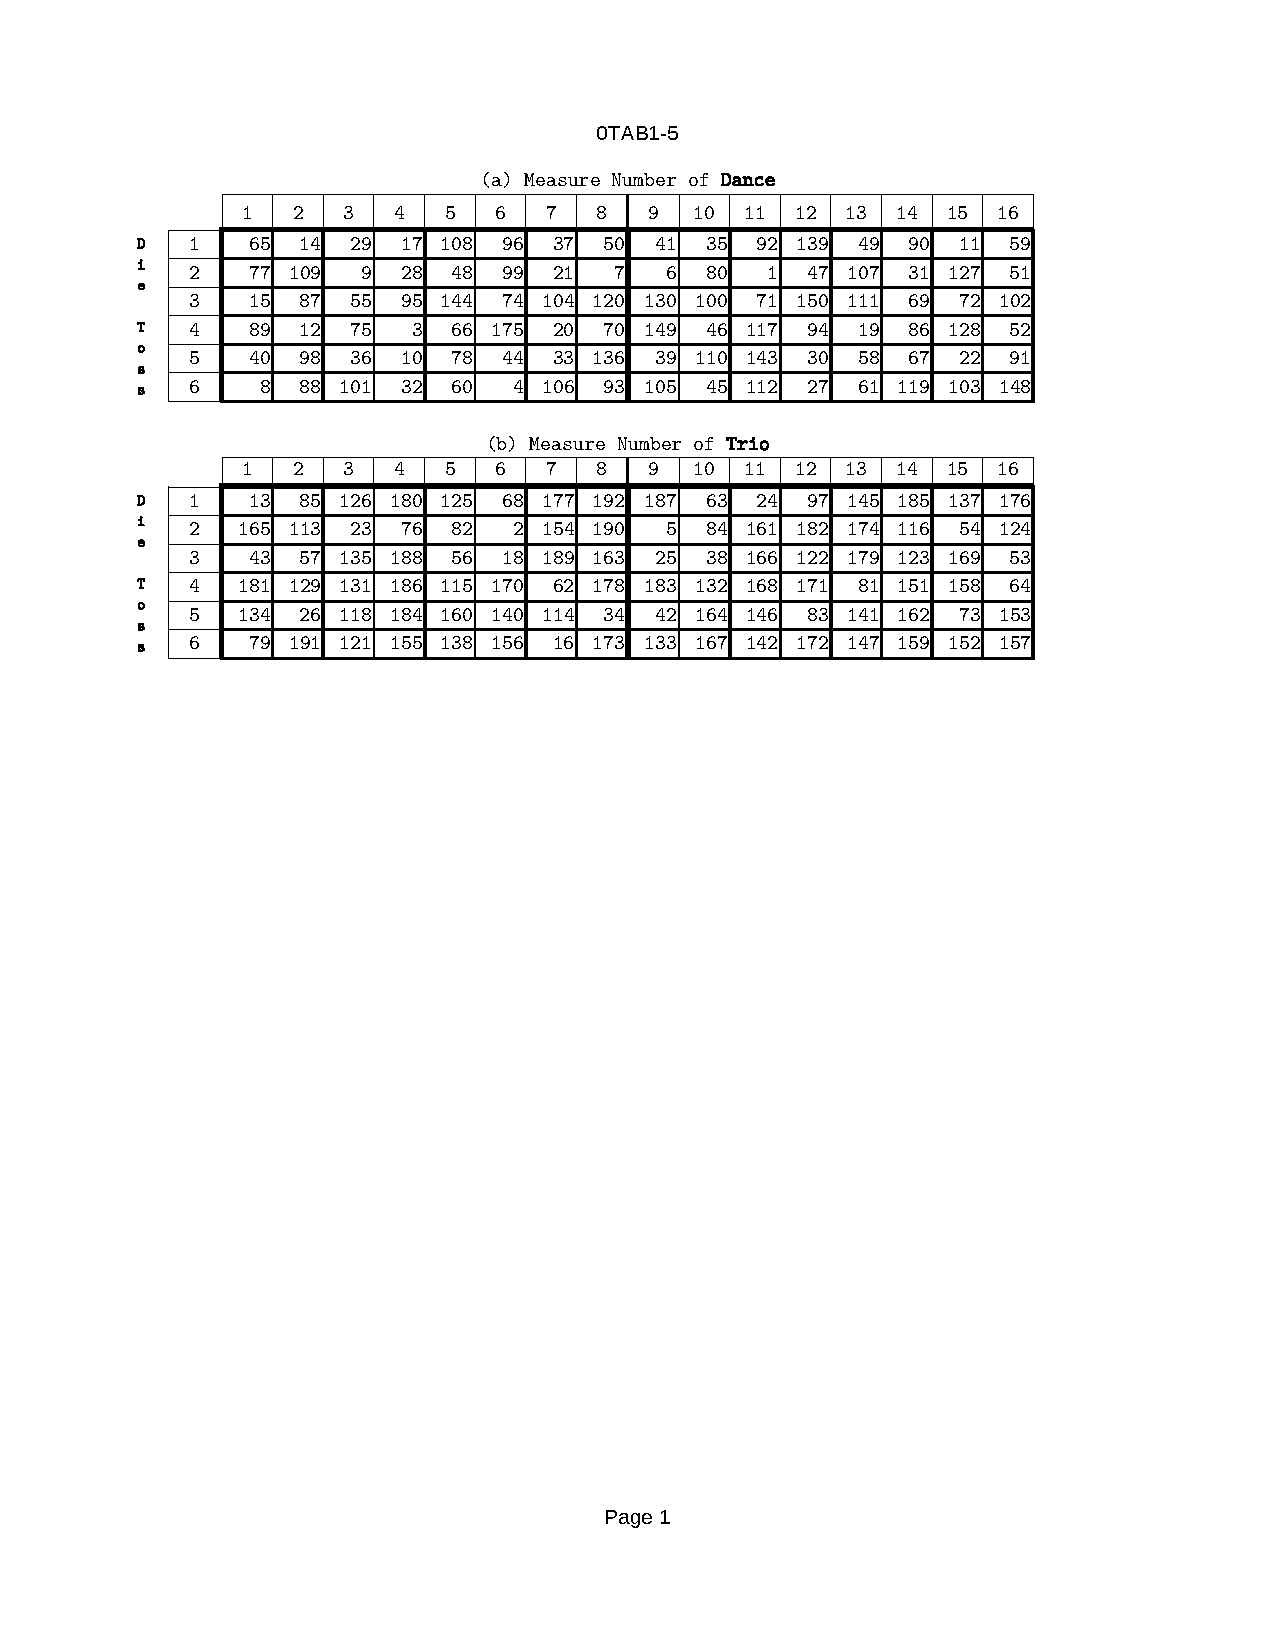
\includegraphics[clip=true,trim=0.75in 6.50in 1.50in 1.10in,scale=0.90]{sd-TAB}
	\end{tabular}
	\caption{This Table of Measures gives the measure number to be looked-up in the Table of Measures (see Figures~\ref{fig:meas1}, \ref{fig:meas2}, \ref{fig:meas3}, and \ref{fig:meas4} in Section~\ref{tabMeas}) corresponding to each one-die outcome per measure for (a) the 16 bars of the Dance and (b) the 16 bars of the Trio (see  \href{https://opus-infinity.org/dice_games/gerlach_scottish_dance/tables/}{https://opus-infinity.org} for more info).}
	\label{fig:0tab1}
\end{table}


\subsection{Table of Measures}\label{tabMeas}

The Table of Measures given in {\em Schottische Taenze} are given in Figures~\ref{fig:meas1}, \ref{fig:meas2}, \ref{fig:meas3}, and \ref{fig:meas4} that follow.  These are based but not exactly identical to those that are given in the last four (4) pages of Gustav Gerlach's \href{https://imslp.org/wiki/Kunst\%2C\_Schottische\_Taenze\_zu\_componiren\%2C\_ohne_musicalisch\_zu\_sein\_(Gerlach\%2C\_Gustav)}{{\em Schottische Taenze}} and the  \href{https://opus-infinity.org/dice_games/gerlach_scottish_dance/measures/}{Table of Measures} published online at  \href{https://opus-infinity.org}{Opus Infinity}.

\newpage
${}_{}$\\
\vspace{0.10in}
\addcontentsline{toc}{subsection}{\hspace*{0.25in} {\em Schottische Taenze} page 1 of measures}	
\begin{figure}[H]
	\centering
	\def\svgwidth{0.975\columnwidth}
	\input{gerlach-schottische001.pdf_tex}
	\caption{Table of Measures (Part 1)}
	\label{fig:meas1}
\end{figure}

\newpage
${}_{}$\\
\vspace{0.10in}
\addcontentsline{toc}{subsection}{\hspace*{0.25in} {\em Schottische Taenze} page 2 of measures}	
\begin{figure}[H]
	\centering
	\def\svgwidth{0.975\columnwidth}
	\input{gerlach-schottische002.pdf_tex}
	\caption{Table of Measures (Part 2)}
	\label{fig:meas2}
\end{figure}

\newpage
${}_{}$\\
\vspace{0.10in}
\addcontentsline{toc}{subsection}{\hspace*{0.25in} {\em Schottische Taenze} page 3 of measures}	
\begin{figure}[H]
	\centering
	\def\svgwidth{0.975\columnwidth}
	\input{gerlach-schottische003.pdf_tex}
	\caption{Table of Measures (Part 3)}
	\label{fig:meas3}
\end{figure}

\newpage
${}_{}$\\
\vspace{0.10in}
\addcontentsline{toc}{subsection}{\hspace*{0.25in} {\em Schottische Taenze} page 4 of measures}	
\begin{figure}[H]
	\centering
	\def\svgwidth{0.975\columnwidth}
	\input{gerlach-schottische004.pdf_tex}
	\caption{Table of Measures (Part 4)}
	\label{fig:meas4}
\end{figure}


%\newpage
\section{Related Links}
The following are very interesting sites in that they allow the online rendering of MDGs:
\begin{itemize}
	\item \href{https://opus-infinity.org}{Opus Infinity} - Collaborative work of Robbert Harms, Hein Moors, and Suus van Petegem whose goal is to unravel the mystery behind the tables used for generating MDGs.  Site visitors can generate MDGs based on works of Kirnberger, Mozart, Stadler/Haydn, Bach, and Gerlach.  Corresponding audio files ({\tt mid, ogg,} and/or {\tt mp3}) and image files ({\tt pdf} or {\tt png}) are also made available for listening, viewing, or downloading.
	
	\item  \href{http://sunsite.univie.ac.at/Mozart/dice/}{Mozart} - A site maintained by John Chuang that allows the site visitor to generate MDGs based on the work of Stadler/Haydn.
	
	\item  \href{https://marian-aldenhoevel.de/mozart/}{Mozart} - A site maintained by Marian Aldenh\"{o}vel allows the visitor to generate a MDG (user-specified or randomly-generated) and the corresponding audio ({\tt midi, wav}) and image files ({\tt pdf, png}) based on {\em Musikalisches W\"{u}rferspiel, K.\ 516f}.
	
	\item \href{https://www.amaranthpublishing.com/mozart.zip}{\tt mozart.zip} -  This is a Windows software ({\small\textcopyright} 1995 VisionSoft) by John Chuang and Stephen Goodwin that generates MDG based on input from user and is available for {\it free} from  \href{http://www.amaranthpublishing.com/MozartDiceGame.htm}{Amaranth Publishing}.  
	
	\item \href{(http://www.asahi-net.or.jp/\~rb5h-ngc/e/k516f.htm}{``Mozart - Musical Game in C K. 516f,"}	Mozart Studies Online - The site of Hideo Noguchi that offers an explanation linking {\em Musikalisches W\"{u}rferspiel, K.\ 516f}, and  {\em K.\ 294d (K.\ Anh.\ C 30.01)}. 
\end{itemize}

\newpage
\section{Acknowledgments}
Special thanks to \href{https://imslp.org}{International Music Score Library Project} for \href{https://imslp.org/wiki/Kunst\%2C\_Schottische\_Taenze\_zu\_componiren\%2C\_ohne_musicalisch\_zu\_sein\_(Gerlach\%2C\_Gustav)}{\it Kunst, Schottische Taenze zu componiren, ohne musicalisch zu sein}, \href{https://opus-infinity.org}{Opus Infinity} for additional related information, and \href{http://www.amaranthpublishing.com/MozartDiceGame.htm}{Amaranth Publishing} for a copy of {\tt mozart.zip}. My sincerest gratitude to Chris Walshaw et al. for the \href{http://www.abcnotation.com/}{ABC music notation}; Jean-Francois Moine for \href{http://moinejf.free.fr/}{\tt abcm2ps} and the accompanying examples, templates, and pointers for the appropriate use of these resources; Guido Gonzato for the \href{http://abcplus.sourceforge.net/}{ABC Plus Project} and the \href{http://abcplus.sourceforge.net/#abcMIDI}{{\tt abcmidi} resources} available there, more especially for the ABC resource book {\em Making Music with ABC 2}; James R. Allwright and Seymour Shlien for \href{http://abc.sourceforge.net/abcMIDI}{\tt abcmidi} source and binaries; \href{https://artifex.com/}{Artifex, Inc.} for Ghostscript v.10.00.0 (includes the {\tt ps2pdf} converter); \href{https://www.inkscape.org/}{Inkscape v.1.2.2} for the tool for converting SVGs to PDFs for inclusion into \LaTeX\ documents; William Schelter for \href{https://maxima.sourceforge.io}{Maxima v.5.47.0}---used for computing the permutation number; Colomban Wendling et.\ al for \href{https://www.geany.org}{Geany 2.0 IDE}; and \href{https://tex.stackexchange.com/users/632/martin-h}{\tt User:Martin H} for his \href{https://tex.stackexchange.com/questions/2099/how-to-include-svg-diagrams-in-latex}{reply} to a \TeX\ / \LaTeX\ Stack Exchange question on including SVGs into \LaTeX\ documents. Thanks to  Ditto to Machtelt Garrels for the book \href{http://tldp.org/LDP/Bash-Beginners-Guide/html/Bash-Beginners-Guide.html}{Bash Guide for Beginners}, Vivek Gite for the book \href{http://www.freeos.com/guides/lsst/}{Linux Script Shell Tutorial}, and Steve Parker for the \href{http://steve-parker.org/sh/cheatsheet.pdf}{Unix/Linux Shell Cheatsheet}. John Fogarty's GitHub Site: \href{https://github.com/jfogarty/latex-createspace-bookcover}{Latex CreateSpace BookCover} and Peter Wilson's reply in  \TeX\ / \LaTeX\ Stack Exchange on \href{https://tex.stackexchange.com/questions/17579/how-can-i-design-a-book-cover}{designing a book cover}, were sources of ideas, information, and materials for creating the book cover and title page, thanks to both of them; \href{http://www.libreoffice.org/}{LibreOffice Calc} for its use in the image creation of the book cover.  Many thanks, too, to the \href{https://www.debian.org}{Debian Project} for the Debian 12 (Bookworm) GNU/Linux OS, \href{http://www.tug.org/texlive/}{TeXLive} for providing the \TeX\ distribution,  and \href{https://github.com}{GitHub} for its generosity in providing space for \href{https://github.com/justineuro/mdgBookSVG6Kit}{the project}.  

%\newpage
\section{Twenty (20) Selected Waltzes}
\vspace{-.10in}
This section contains an example of 20 SDs that were generated using the Rules in Section~\ref{mdgRules}.
\vspace{-.10in}
{
\topmargin -1.00in
\textheight 10.5in
\input{svgList}
}	

\newpage
\section{License}
This work by I Am The Author, based on work of J.L.A. Uro at  \url{https://github.com/justineuro/mdgBookSVG6Kit}, is licensed under a Creative Commons Public Domain International License.

\bibliographystyle{plainnat}
\bibliography{mdg6}

 

\end{document}
